\documentclass[../norme-di-progetto.tex]{subfiles}

\begin{document}

\subsection{Descrizione}%
\label{sub:descrizione}

I processo di supporto operano a sostegno degli altri processi con lo scopo di garantire il successo e fornire qualità. Essi non esistono autonomamente ma hanno la necessità di appoggiarsi ad altri processi. ISO 11207-1995 ne distingue otto:

\begin{itemize}
  \item Documentazione
  \item Gestione della configurazione
  \item Accertamento della qualità
  \item Verifica
  \item Validazione
  \item Revisioni congiunte
  \item Verifiche interne
  \item Risoluzione dei problemi
\end{itemize}

\subsection{Documentazione}%
\label{sub:documentazione}

\subsubsection{Finalità}%
\label{subs:finalità}

Grupp0ne istanzia il processo di documentazione per illustrare in maniera chiara e coerente le attività di processo svolte e i prodotti da esse ottenuti.

\subsubsection{Descrizione}%
\label{subs:descrizione}

La documentazione è essenziale durante ogni attività del ciclo di vita del software.
Essa costituisce un importante mezzo di comunicazione sia internamente per il team che esternamente verso il committente.
Si vogliono quindi definire delle norme che possano standardizzare il processo di documentazione e renderlo più accessibile a tutti i componenti del gruppo.

\subsubsection{Implementazione}%
\label{subs:implementazione}

\paragraph{Configurazione} \mbox{}\\
\label{par:configurazione}
\\Ogni documento ha una sua configurazione di base. Tale configurazione è definita in un file \LaTeX  che contiene la struttura e la formattazione che ogni file deve avere. Si riporta un elenco di ciò che è presente nel file di configurazione:

\begin{itemize}
  \item Definizione e decorazione di header e footer.
  \item Definizione dei margini laterali e dell'altezza del footer.
  \item Setup della sottolineatura delle parole.
  \item Configurazione dei link.
  \item Dichiarazione di nuovi comandi.
\end{itemize}

\paragraph{Ciclo di vita}\mbox{}\\
\label{par:ciclo di vita}
\\Il ciclo di vita di rappresenta gli stadi in cui il documento si può trovare nel corso della sua esistenza. Ne distinguiamo cinque:
\begin{description}
  \item [Creazione del template del documento]: un membro del gruppo crea il template del documento il quale conterrà solamente una pagina di frontespizio. Inizialmente sono configurate una serie di impostazioni di base per la formattazione delle pagine grazie all'utilizzo di alcuni package di \LaTeX.
  \item [Scrittura del documento]: l'incaricato scrive il documento incrementalmente e lo termina entro la scadenza della \glossario{milestone} fissata.
  \item [Verifica del documento]: i \glossario{verificatori} effettuano una revisione del documento segnalando eventuali errori o discordanze che verranno segnalate all'autore del documento che sarà incaricato di correggerli.
  \item [Approvazione del documento]: il \glossario{responsabile} di progetto approva il documento.
  \item [Archiviazione]: l'amministratore archivia il documento in un repository pubblico su \glossario{github}.
\end{description}
\subsubsection{Struttura}
\label{subs:struttura}

\paragraph{Frontespizio}\mbox{}\\
\label{par:frontespizio}
\\Il frontespizio è la prima pagina di ogni documento. È diviso in due parti: nella prima è presente l'intestazione contenente logo, nome del gruppo e nome del documento, mentre la seconda consiste di uno schema contenente alcune informazioni essenziali sul documento descritto. In esso compaiono, ordinatamente, dall'alto verso il basso:

\begin{itemize}
  \item Intestazione
  \begin{itemize}
    \item \textbf{Logo}: rappresenta il logo del team.
    \item \textbf{Nome del gruppo}: rappresenta il nome del gruppo.
    \item \textbf{Nome del documento}: rappresenta nome del documento.
  \end{itemize}
  \item Schema
  \begin{itemize}
    \item \textbf{Versione}: indica la versione attuale del documento (e.g. glossario v1.0.0).
    \item \textbf{Approvazione}: indica chi ha approvato il documento.
    \item \textbf{Redazione}: indica la lista dei redattori del documento.
    \item \textbf{Verifica}: indica la lista dei verificatori del documento.
    \item \textbf{Stato}: indica lo stato attuale in cui si trova il documento.
    \item \textbf{Uso}: indica l'uso finale del documento (interno o esterno).
    \item \textbf{Destinato a}: indica lo stato attuale del documento.
    \item \textbf{Descrizione}: indica una breve descrizione del documento.
  \end{itemize}
\end{itemize}

\paragraph{Registro delle modifiche}\mbox{}\\
\label{par:registro delle modifiche}
\\Il registro delle modifiche è la seconda pagina di ogni documento. Ha lo scopo di presentare quali cambiamenti sono stati effettuati e da parte di quale componente del gruppo. Consiste di quattro colonne ed è così articolato:
\begin{description}
  \item [Versione]: indica la versione del documento in cui viene realizzata la modifica.
  \item [Data]: indica la data di modifica del documento con formato yyyy/mm/dd.
  \item [Nominativo]: indica nome e cognome del componente del team che ha effettuato la modifica.
  \item [Ruolo]: indica il ruolo del componente del team che ha realizzato la modifica.
  \item [Descrizione]: indica il tipo e il luogo in cui è avvenuta la modifica.
\end{description}
\paragraph{Indice}\mbox{}\\
\label{par:indice}
\\L'indice inizia nella terza pagine del documento e presenta tutti gli argomenti trattati. Grupp0ne ha deciso di utilizzare la tipica suddivisione del testo offerta da \LaTeX che distingue cinque diversi blocchi testuali:

\begin{itemize}
  \item Sezioni
  \item Sottosezioni
  \item Sotto-sottosezioni
  \item Paragrafi
  \item Sottoparagrafi
\end{itemize}
Ogni blocco testuale ha un numero identificativo univoco la cui lunghezza dipende dal grado di annidamento del blocco che è predefinita da \LaTeX (e.g.:\ la sezione Introduzione è indicata con 1, la relativa sottosezione quattro è indicata con 1.4 e i capitoli contenuti in quella sottosezione sono indicati con 1.4.1 e 1.4.2).
% TODO sistemare \newline?
\newline Ogni riga dell'indice contiene il numero di pagina in cui il blocco di testo è riferito e cliccando sopra il nome del blocco è possibile raggiungerlo direttamente attraverso un link.

\paragraph{Contenuto}\mbox{}\\
\label{par:contenuto}
\\Le pagine di contenuto sono suddivise in tre parti:
\begin{description}
  \item [Header]: contiene in alto a sinistra il logo del gruppo, mentre in alto a destra il nome del documento.
  \item [Contenuto]: contiene il testo del documento.
  \item [Footer]: contiene l'indicazione della pagina attuale rispetto il totale (e.g 1/6).
\end{description}
\paragraph{Norme per la redazione dei documenti}
\label{par:norme per la redazione dei documenti}
\subparagraph{Stile del testo}\mbox{}\\
\label{subp:stile del testo}
\\In questo paragrafo Grupp0ne definisce le norme che uniformano lo stile di scrittura dei documenti:
\begin{description}
    \item [Verbi in forma attiva]: i verbi devono essere in forma attiva e al tempo presente indicativo o passato prossimo. È ammesso l'uso del futuro per esprimere azioni che devono ancora avvenire.
    \item [Struttura del testo chiara]: la suddivisione del testo in sezioni, sottosezioni e paragrafi aiuta la coerenza e la coesione.
    \item [Frasi brevi e poco complesse]: i periodi devono essere il più possibile semplici per non generare incomprensioni.
    \item [Uso degli elenchi puntati]: per evitare lunghe digressioni ed eccessiva verbosità si vogliono utilizzare gli elenchi puntati laddove è possibile.
    \item [Brevi blocchi testuali]: si preferisce l'utilizzo di brevi paragrafi.
    \item [Termini di glossario in maiuscolo]: il testo è scritto in minuscolo. I termini di glossario, invece, sono indicati in maiuscolo con una g a pedice nel nome. Questa regola vale per la prima occorrenza di ogni termine di glossario.
\end{description}
\subparagraph{Elenchi puntati}\mbox{}\\
\label{subp:elenchi puntati}
\\Gli elenchi puntati sono un mezzo ottimo per la scrittura di documentazione. Essi permettono di riordinare il testo e di elencare una serie di elementi correlati. Pertanto, in questo paragrafo, si stabiliscono le norme per il corretto uso degli elenchi puntati:

\begin{enumerate}
  \item Per indicare gli elementi di un elenco puntato non innestato utilizzare il simbolo •. Gli elementi innestati vengono preceduti da -.
  \item Ogni elemento di elenco puntato inizia con una lettera maiuscola.
  \item Se un elenco puntato ha elementi composti da etichetta e descrizione, l'etichetta deve essere scritta in grassetto e la descrizione va inserita dopo i due punti.
  \item Gli elenchi puntati semplici non hanno bisogno di punti fermi per terminare la frase. Gli elenchi puntati complessi in particolare quelli formati da etichetta e descrizione richiedono un punto al termine della descrizione.
\end{enumerate}

\subparagraph{Nomi dei file}\mbox{}\\
\label{nomi dei file}
\\Per identificare i file memorizzati nel repository si seguono le seguenti convenzioni:

\begin{itemize}
  \item I nomi dei file devono essere in minuscolo.
  \item Le parole contenute nei nomi di file composti devono essere separate da -.
\end{itemize}

Analisi dei requisiti sarà quindi salvato come analisi-dei-requisiti, mentre Norme di progetto come norme-di-progetto.

\subparagraph{Sigle e convenzioni}\mbox{}\\
\label{sigle e convenzioni}
\\Si elencano una serie di sigle che possono essere utilizzate nei documenti. Si accompagna ad ognuna di esse il relativo significato:

\begin{itemize}
  \item sigle per identificare le revisioni
  \begin{itemize}
    \item \textbf{RR}: revisione dei requisiti
    \item \textbf{RP}: revisione di progettazione
    \item \textbf{RQ}: revisione di qualifica
    \item \textbf{RA}: revisione di accettazione
  \end{itemize}
  \item sigle per identificare i documenti
  \begin{itemize}
    \item \textbf{AdR}: analisi dei requisiti
    \item \textbf{NdP}: norme di progetto
    \item \textbf{PdQ}: piano di qualifica
    \item \textbf{PdP}: piano di progetto
    \item \textbf{MU}: manuale utente
    \item \textbf{MS}: manuale sviluppatore
    \item \textbf{V}: verbali
   \end{itemize}
 \end{itemize}
\subparagraph{Immagini}\mbox{}\\
\label{subp:immagini}
\\Le immagini si devono utilizzare per apportare un valore aggiunto a ciò che si sta descrivendo o per dare una rappresentazione grafica di ciò che si sta presentando.
Immagini di bellezza non sono pertanto ammesse.
Tutte le immagini devono essere inoltre centrate all'interno della pagina e munite di una breve didascalia così formata: \\\\\centerline{\textbf{Figura x : breve descrizione dell'immagine}} \\\\ dove x indica la numerazione delle immagini (e.g. figura 1, figura 2, figura 3).

\subparagraph{Tabelle}\mbox{}\\
\label{subp:tabelle}
\\L'uso di tabelle è consigliato solo quando strettamente necessario. La rappresentazione dei dati in forma tabellare è obbligatoria solo nel momento in cui risulti molto difficile organizzare informazioni aventi una struttura complessa. È obbligatorio l'uso di colori che abbiano un elevato contrasto al fine di promuovere la leggibilità. Inoltre, non devono essere eccessivamente lunghe ( massimo 2 pagine), altrimenti risultano dispersive.
\subsubsection{Produzione}
\paragraph{Suddivisione dei documenti}\mbox{}\\
\\I documenti utilizzano la struttura a \glossario{subfiles} offerta da \LaTeX. La struttura di base del documento è definita nel file che porta il nome del documento. La cartella components, che è unica per ogni documento, contiene un file per la definizione di ogni sezione. In ogni sezione si definiscono poi le relative sottosezioni, paragrafi e sottoparagrafi.
Ad esempio, il file norme di progetto ha la seguente struttura:

\begin{itemize}
  \item ..\textbackslash interni
  \begin{itemize}
  \item Norme di progetto
     \begin{itemize}
       \item norme-di-progetto.tex
       \item components
       \begin{itemize}
         \item processi-primari.tex
         \item processi-di-supporto.tex
         \item introduzione.tex
         \item processi-organizzativi.tex
       \end{itemize}
     \end{itemize}
  \item Studio di fattibilità
  \end{itemize}
\end{itemize}

\subparagraph{Interni}\mbox{}\\
\label{subp:interni}
\\ I documenti interni sono destinati alla comunicazione tra i componenti di Grupp0ne. Appartengono a tale categoria:

\begin{itemize}
  \item Verbali interni
  \item Studio di fattibilità
  \item Norme di progetto
\end{itemize}

\subparagraph{Esterni}\mbox{}\\
\label{subp:esterni}
\\ I documenti esterni sono destinati al committente. Appartengono a tale categoria:

\begin{itemize}
  \item Analisi dei requisiti
  \item Piano di progetto
  \item Piano di qualifica
\end{itemize}

\subparagraph{Verbali}\mbox{}\\
\label{subp:verbali}
\\ I verbali contengono un riassunto degli incontri di Grupp0ne. Se qualche componente del gruppo non fosse presente a un incontro è necessario che prenda visione del relativo verbale in modo che possa informarsi su cosa è stato discusso alla riunione in cui era assente. I verbali sono così costituiti:
\begin{description}
  \item [Titolo]: il titolo indica che il documento in questione è un verbale e mostra la data di redazione.
  \item [Schema]: lo schema contiene le informazioni basilari relative al documento. È identico allo schema degli altri documenti, spiegato nella sezione \ref{par:frontespizio}.
  \item [Ordine del giorno]: l'ordine del giorno consiste in un elenco puntato degli argomenti che saranno trattati nel verbale. Ogni elemento dell'elenco verrà sviluppato in una sezione del documento che potrà contenere altre sottosezioni, paragrafi o sottoparagrafi.
\end{description}
\subsubsection{Strumenti}
\paragraph {\LaTeX}\mbox{}\\
\label{par:LaTeX}
\\ \LaTeX  è lo strumento utilizzato da Grupp0ne per la stesura: si è preferito non utilizzare dei tool online per la scrittura dei documenti. Ogni componente del gruppo ha scaricato, invece, un' estensione per il proprio IDE preferito( sublime text o Visual Studio Code) che consentisse l'installazione dei principali package di \LaTeX e che garantisse correttamente l'esecuzione del processo di build dei file .tex.
\subsection{Gestione della configurazione}
\label{sub:gestione della configurazione}
\subsubsection{Finalità}
\label{subs:finalità}
\subsubsection{Gestione versionamento}
\label{subs:gestione versionamento}

\paragraph{Repository}\mbox{}\\
\label{par:repository}

\paragraph{Struttura dei commit}\mbox{}\\
\label{par:struttura dei commit}

\subsubsection{Strumenti}%
\label{subs:strumenti}
\subsection{Accertamento della qualità}
\label{sub:accertamento della qualità}

\subsubsection{Finalità}
\label{subs:finalità}
Grupp0ne istanzia il processo di accertamento della qualità per garantire qualità di processo e di prodotto. Gli esiti dei processi di verifica e validazione saranno indispensabili al buon svolgimento del processo di accertamento della qualità.
\subsubsection{Descrizione}
\label{subs:descrizione}
Il processo di accertamento della qualità garantisce che i prodotti e i processi del ciclo di vita del software rispettino i requisiti e che aderiscano ai piani esecutivi prestabiliti. Le metriche e gli strumenti per valutare la qualità sono presentati nel \glossario{piano di qualifica}.
\subsubsection{Attività}
\label{subs:attivita}
Le principali attività coinvolte nel processo di accertamento della qualità sono:
\begin{description}
  \item [Pianificazione]: si cercano le metodologie, le procedure, gli strumenti e anche le attività offerte da altri processi di supporto per organizzare le pianificazione della qualità.
  \item [Implementazione]: si utilizza ciò che si è individuato al passo 1 per effettuare controlli di qualità sui processo in atto e sui prodotti in atto.
  \item [Documentazione dei risultati]: i risultati dei controlli di qualità dovrebbero essere poi documentati.
\end{description}
\paragraph{Accertamento qualità di prodotto}\mbox{}\\
\label{par:accertamento qualita di prodotto}
\\L'attività di accertamento della qualità di prodotto vigila sulla qualità dei prodotti realizzati. Essa promuove controlli continui che possano prevenire danni irreparabili al termine del progetto. È fortemente dipendente dalla qualità di processo: da processi privi di qualità, infatti, non è possibile ottenere buoni prodotti.
\paragraph{Accertamento qualità di processo}\mbox{}\\
\label{par:accertamento qualita di processo}
\\L'attività di accertamento della qualità di processo monitora i processi istanziati. Per avere un sistema di accertamento della qualità di processo che funzioni è necessario che:

\begin{itemize}
  \item Si individuino i processi da controllare
  \item Si stabiliscano le metriche di valutazione del processo
  \item Si eseguano accertamenti continui sui processi scelti
  \item In base ai risultati ottenuti, si ricerchi un miglioramento dei processi
\end{itemize}

\subparagraph{PDCA}\mbox{}\\
\label{subp:PDCA}
\\Il ciclo deming o ciclo di PDCA è un processo iterativo per il monitoraggio e il miglioramento di processo. Sfrutta la ripetizione di quattro attività:
\begin{description}
  \item [Plan]: definisce gli obiettivi, le attività e i processi necessari per raggiungere i risultati attesi.
  \item [Do]: esegue ciò che è stato definito nella fase di pianificazione.
  \item [Check]: verifica gli esiti dei processi.
  \item [Act]: esegue azioni correttive per migliorare la qualità dei processi.
\end{description}
\begin{figure}[H]
  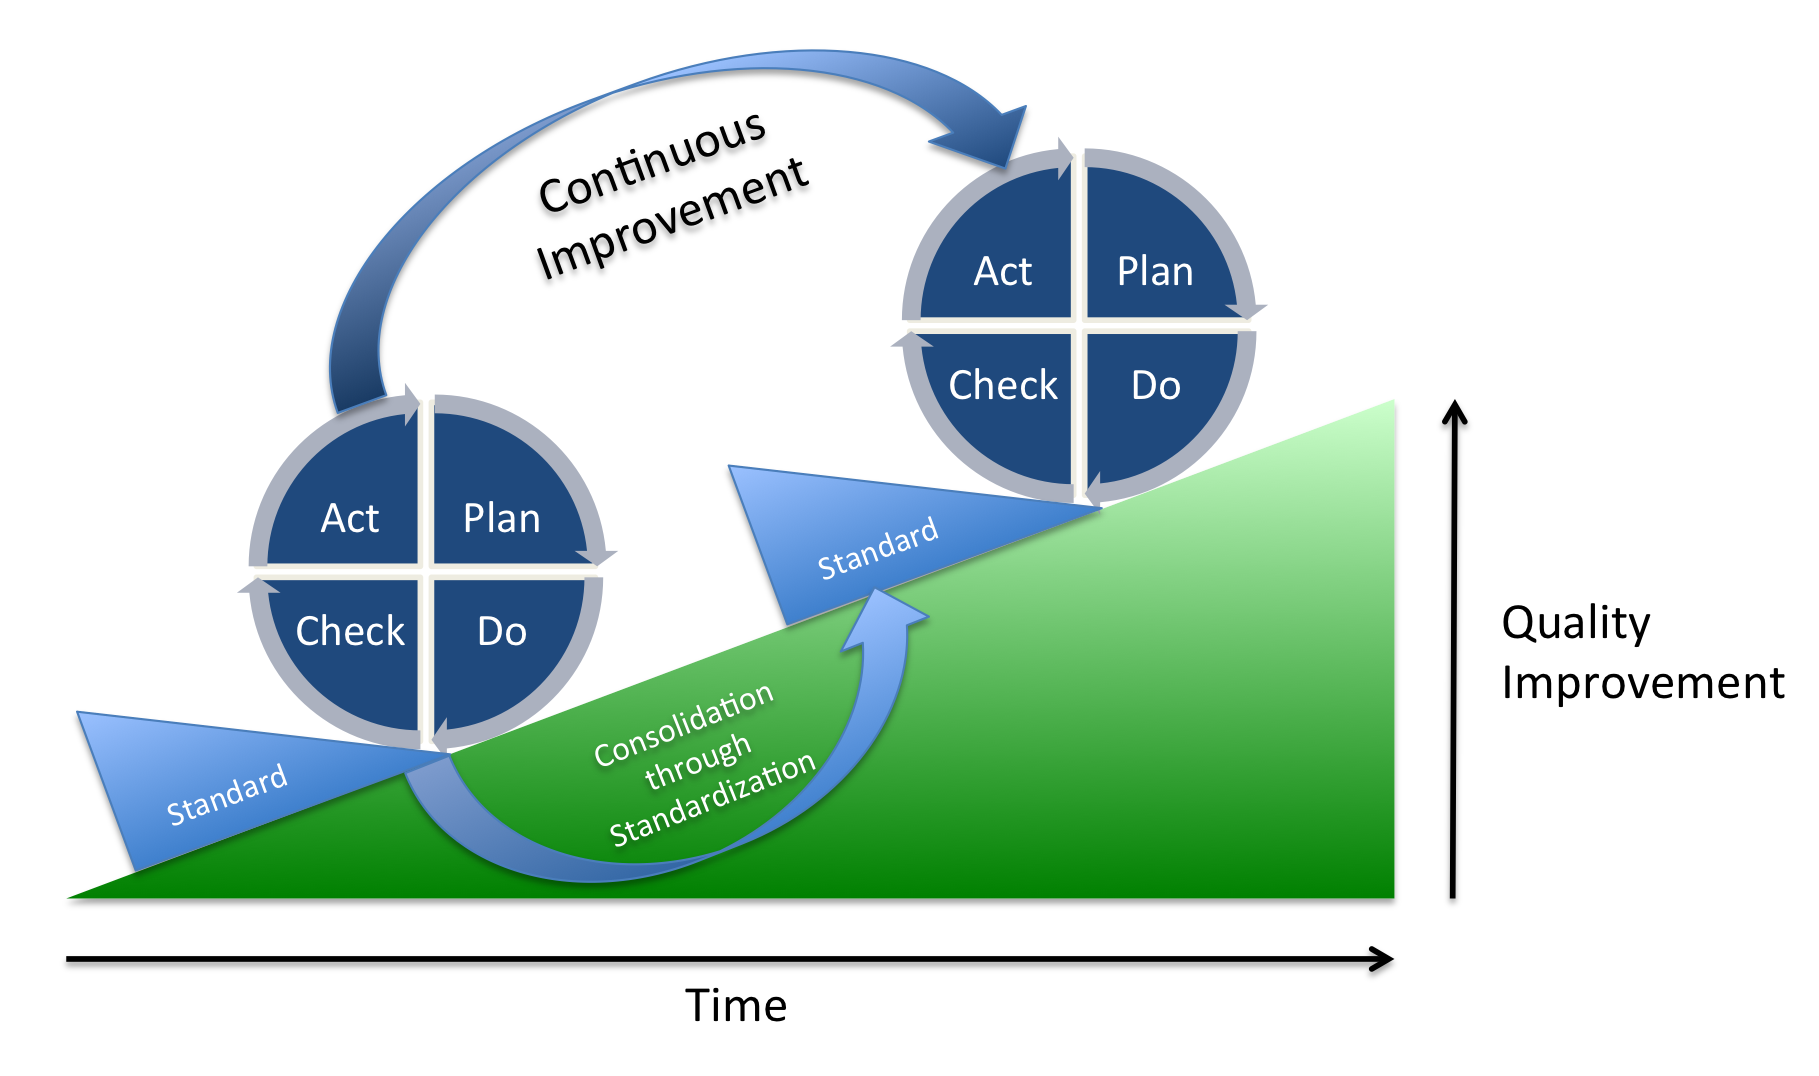
\includegraphics[width=8cm]{components/PDCA-process.png}
  \centering
  \caption{ciclo di Deming o PDCA.}
\end{figure}

% TODO aggiungere label mancante
\subsection{Verifica}
\label{sub:verifica}
\subsubsection{Finalità}
\label{subs:finalità}
Grupp0ne istanzia il processo di verifica  per certificare che il susseguirsi di attività diverse non comporti l'introduzione di errori nei prodotti intermedi.
Si deve verificare qualsiasi prodotto intermedio, pertanto sia documentazione che codice sono soggetti a verifica
\subsubsection{Descrizione}

Il processo di verifica è il processo che controlla e garantisce che i prodotti di una determinata attività soddisfino i requisiti e le condizioni che quel prodotto deve avere. Il processo di verifica si integra in toto con gli altri processi, in particolare con quello di sviluppo e offre attività di revisione, analisi e test. È composto da due attività:

\begin{itemize}
  \item Implementazione di processo
  \item Verifica
\end{itemize}

\paragraph{Analisi statica}\mbox{}\\
\label{par:analisi statica}
\\L'analisi statica fornisce l'insieme delle buone pratiche che valutano un componente del sistema sulla base della sua forma, struttura e contenuto. L'analisi statica quindi definisce una serie di regole  a cui tutti i prodotti intermedi del ciclo di vita del software devono attenersi. Esistono due tipi di analisi statica:
\begin{description}
  \item [Walkthrough]: La tecnica walkthrough esegue una verifica a largo spettro del prodotto. Si articola nelle seguenti attività:
  \begin{itemize}
    \item Pianificazione di cosa è necessario monitorare.
    \item Lettura dell'oggetto di verifica da parte di più membri del team.
    \item Discussione dei difetti individuati da tutti i componenti del team.
    \item Correzione concordata degli errori trovati.
  \end{itemize}
  \item [Inspection]: l'inspection esegue una verifica mirata del prodotto. Si articola nelle seguenti attività:
  \begin{itemize}
    \item Pianificazione di cosa è necessario monitorare.
    \item Costruzione di una checklist di controllo.
    \item Lettura dell'oggetto di verifica sulla base delle metriche definite nella lista di controllo.
    \item Correzione degli errori trovati.
  \end{itemize}
\end{description}
Grupp0ne predilige la tecnica inspection pertanto si impegna a fornire una checklist dei controlli da effettuare sui documenti e sul software.

\subparagraph{Analisi statica dei documenti}\mbox{}\\
\label{subp:analisi statica dei documenti}
\\ Di seguito si riporta una checklist da seguire per effettuare l'analisi statica dei documenti:
\begin{description}
    \item [Errori di ortografia]: si devono individuare errori di punteggiatura.
    \item [Errori nei verbi]: si deve controllare che tutti i verbi siano in forma attiva.
    \item [Errori di sintassi]: si deve verificare che non ci siano paragrafi di lunghezza eccessiva e che le frasi siano il più brevi possibile.
    \item [Errori negli elenchi puntati]: si deve controllare che ogni elemento di elenco puntato inizi con la lettera maiuscola e che vengano rispettate le regole definite in \ref{subp:elenchi puntati}.
    \item [Errori nella strutturazione del documento]: si deve verificare che tutti i paragrafi si trovino nella sezione corretta, che le sezioni siano ben strutturate e che i titoli siano significativi.
\end{description}
Sarà compito dei verificatori attenersi alla checklist definita in \ref{subp:analisi statica dei documenti} per le attività di verifica.

\paragraph{Analisi dinamica del codice}\mbox{}\\
\label{par:analisi dinamica del codice}
\\L'analisi dinamica del codice necessita che l'oggetto di verifica sia in esecuzione. Essa cerca di dimostrare che il programma svolge i compiti per il quale è stato realizzato e identifica gli errori prima che il software sia messo in uso. Si realizza attraverso la creazione e l'esecuzione di test che producono deterministicamente un risultato da confrontare con un valore atteso. Il numero di test è chiaramente finito e quindi non sarà possibile provare tutte le esecuzioni possibili. Per questo motivo bisogna produrre dei test sensati. Un test affinchè sia definito come tale deve avere delle precise caratteristiche:
\begin{itemize}
  \item Velocità
  \item Ripetibilità
  \item Bassa interazione umana
\end{itemize}
\subparagraph{Copertura dei test}\mbox{}\\
\label{subp:copertura dei test}
\\Per ogni tipo di test è necessario fornire la sua copertura. Essa è un valore percentuale e indica quante linee di codice i test hanno esercitato sul totale. Più la copertura è alta meglio è, tuttavia una copertura del 100 \% non dà in alcun modo la certezza di essere in assenza di difetti. Il capitolato di Stalker richiede una copertura dei test pari almeno all' 80 \% corredata da report.
\subparagraph{Test di unità}\mbox{}\\
\label{subp:test di unità}
\\ Il software è un insieme di componenti. Per effettuare verifica del software è necessario adottare un approccio \glossario{bottom-up} che deve necessariamente occuparsi di controllare prima che le unità su cui è costruito il software siano corrette. I test di unità, quindi, servono proprio a testare i moduli elementari del software.
\subparagraph{Test di integrazione}\mbox{}\\
\label{subp:test di integrazione}
\\ I test di integrazione si occupano di verificare l'interazione tra le sottocomponenti del sistema. Essi suppongono che i test di unità siano già stati eseguiti e abbiano dato esito positivo. Lo scopo dei test di integrazione è, pertanto quello di dimostrare che le interfacce delle componenti del software si comportino conformemente alle specifiche richieste.
\subparagraph{Test di sistema}\mbox{}\\
\label{test di sistemaa}
\\ I test di sistema si possono iniziare solo nel momento in cui i test di integrazione abbiano dato esito positivo. Essi verificano il comportamento generale del software rispetto ai requisiti. Durante i test di sistema si esercitano quelle funzionalità di alcune componenti del software che sono fortemente dipendenti da altri moduli del sistema.
\subparagraph{Test di regressione}\mbox{}\\
\label{test di regressione}
\\I test di regressione servono per accertare che modifiche apportate non comportino altri errori nel software: consiste nella ripetizione selettiva di test di unità, test di integrazione, test di sistema.
\subparagraph{Test di accettazione}\mbox{}\\
\label{test di accettazione}
\\I test di accettazione verificano il completo soddisfacimento dei requisiti utente. Sono eseguiti in collaborazione con il committente.
\paragraph{Strumenti}\mbox{}\\
\label{par:strumenti}
\subparagraph{Controllo ortografico e della sintassi}\mbox{}\\
\label{subp:controllo ortografico e della sintassi}
\subparagraph{Code owners}\mbox{}\\
\label{subp:code owners}

\subsection{Validazione}%
\label{sub:validazione}

\subsubsection{Finalità}%
\label{subs:finalità}

Grupp0ne istanzia il processo di validazione per assicurarsi che il prodotto finale realizzato abbia pienamente soddisfatto le attese del committente.

\subsubsection{Descrizione}%
\label{subs:descrizione}

Dovendo verificare se il prodotto finale soddisfa i requisiti, anche il processo di validazione fa uso dell'analisi dinamica del codice e quindi di test ad hoc per dimostrare la correttezza del prodotto.

\subsubsection{Piano di validazione}%
\label{subs:piano di validazione}

Il piano di validazione comprende tutte le attività del processo di validazione:

\begin{itemize}
  \item Scelta dell'oggetto di validazione
  \item Decisione dei compiti da eseguire per realizzare la validazione
  \item Determinazione delle risorse e delle responsabilità
  \item Procedure per fornire al cliente i report di validazione
\end{itemize}

\end{document}